\indent Nos interesa estudiar el comportamiento de nuestro algoritmo frente a la problematica planteada, elaboramos diversos tests que ser\'an enunciados a continuaci\'on.\\

\begin{center}
 \subsubsection*{Caso 1: No existe arbol que conecte todas las salas}
\end{center}

Este caso se da cuando en cualquier camino nos encontramos con paredes irrompibles sin la posibilidad de esquivarlas\\

 Para este tipo de testeo mostraremos a continuaci\'on un ejemplo del mismo.\\
 
\vspace*{0.3cm} \vspace*{0.3cm}
  \begin{center}
 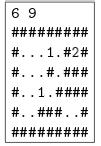
\includegraphics[scale=1.6]{./EJ2/ej2sinsolucion.jpeg}
\\{$Ejemplo$ \ 2.1 - $Caso$ $Sin$ $Soluci$\'on}
  \end{center}
  \vspace*{0.3cm}

El grafo que representa a este tipo es de la siguiente forma:\\

\vspace*{0.3cm} \vspace*{0.3cm}
  \begin{center}
 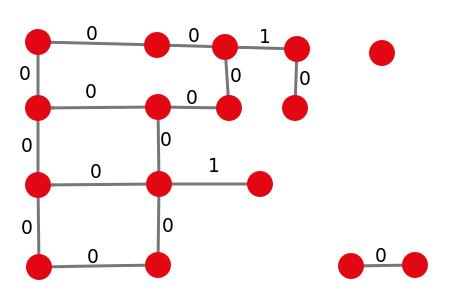
\includegraphics[scale=0.5]{./EJ2/ej2grafosinsolucion.jpeg}
 \\{Representación \ 2.1 - $Caso$ $Sin$ $Soluci$\'on}
  \end{center}
  \vspace*{0.3cm}

 \begin{center}
 \subsubsection*{Caso 2: Existe un camino que conecta todas las salas de esfuerzo 0}
\end{center}

Esta versi\'on se da cuando la suma de los pesos de las aristas del AGM obtenido es 0. 

Para este tipo de testeo mostraremos a continuaci\'on un ejemplo del mismo.\\

\vspace*{0.3cm} \vspace*{0.3cm}
  \begin{center}
 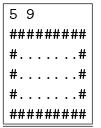
\includegraphics[scale=1.6]{./EJ2/ej2sinpared.jpeg}
 \\{$Ejemplo$ \ 2.2 - $Caso$ $Sin$ $Romper$ $Paredes$}
  \end{center}
  \vspace*{0.3cm}

El grafo que representa a este tipo es de la siguiente forma:\\

\vspace*{0.3cm} \vspace*{0.3cm}
  \begin{center}
 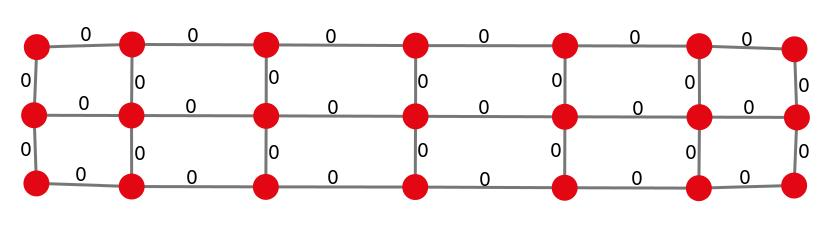
\includegraphics[scale=0.5]{./EJ2/ej2grafosinpared.jpeg}
 \\{Representación \ 2.2 - $Caso$ $Sin$ $Romper$ $Paredes$}
  \end{center}
  \vspace*{0.3cm}
  
\begin{center}
\subsubsection*{Caso 3: El AGM es todo el grafo}
\end{center}

Este caso se da cuando el laberinto no presenta varios caminos para poder ir a las salas sino un \'unico camino.

Aqu\'i veremos, un ejemplo del conjunto de test de este tipo.\\
 
\vspace*{0.3cm} \vspace*{0.3cm}
  \begin{center}
 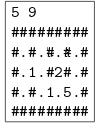
\includegraphics[scale=1.6]{./EJ2/ej2completo.jpeg}
\\ {$Ejemplo$ \ 2.3 - $Caso$ $AGM = GRAFO$}
  \end{center}
  \vspace*{0.3cm}

El grafo que representa a este tipo es de la siguiente forma:\\

\vspace*{0.3cm} \vspace*{0.3cm}
  \begin{center}
 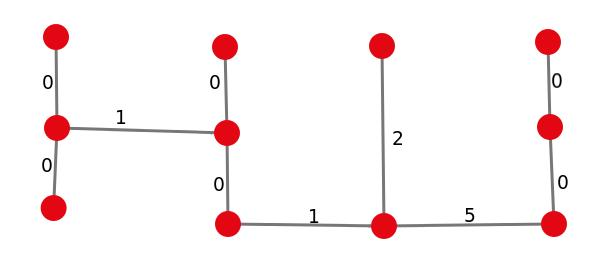
\includegraphics[scale=0.5]{./EJ2/ej2grafocompleto.jpeg}
 \\{Representación \ 2.3 - $Caso$ $AGM = GRAFO$}
  \end{center}
  \vspace*{0.3cm}

\begin{center}
 \subsubsection*{Caso 4: Sin ejes}
\end{center}

Este caso se da cuando todas las salas presentan paredes irrompibles sin la posiblidad de conectarse generando as\'i un grafo sin aristas.\\

Siguiendo el desarrollo de dicho informe a continuaci\'on mostraremos.\\
 
\vspace*{0.3cm} \vspace*{0.3cm}
  \begin{center}
 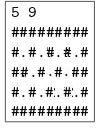
\includegraphics[scale=1.6]{./EJ2/ej2sinejes.jpeg}
\\ {$Ejemplo$ \ 2.4 - $Caso$ $Sin$ $Ejes$}
  \end{center}
  \vspace*{0.3cm}

El grafo que representa a este tipo es de la siguiente forma:\\

\vspace*{0.3cm} \vspace*{0.3cm}
  \begin{center}
 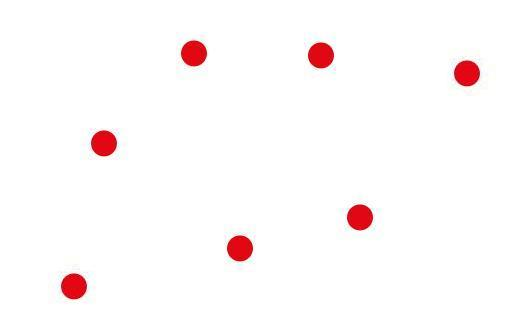
\includegraphics[scale=0.5]{./EJ2/grafoSinEjes.jpeg}
 \\{Representación \ 2.4.2 - $Caso$ $Sin$ $Ejes$}
  \end{center}
  \vspace*{0.3cm}

\begin{center}
 \subsubsection*{Caso 5: Camino por las salas random}
\end{center}

Este caso se da cuando hay posiblidad de conectar todas las salas rompiendo una cierta cantidad de paredes, tambi\'en denominado caso random debido al desarrollo de nuestro algoritmo.\\

Siguiendo el desarrollo de dicho informe a continuaci\'on mostraremos.\\
 
\vspace*{0.3cm} \vspace*{0.3cm}
  \begin{center}
 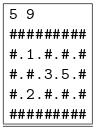
\includegraphics[scale=1.6]{./EJ2/ej2random.jpeg}
\\ {$Ejemplo$ \ 2.5 - $Caso$ $Random$}
  \end{center}
  \vspace*{0.3cm}

El grafo que representa a este tipo es de la siguiente forma:\\

\vspace*{0.3cm} \vspace*{0.3cm}
  \begin{center}
 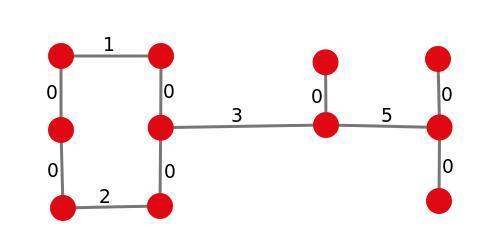
\includegraphics[scale=0.5]{./EJ2/ej2graforandom.jpeg}
 \\{Representación \ 2.5.2 - $Caso$ $Random$}
  \end{center}
  \vspace*{0.3cm}

\textbf{Aclaraciones:} 
\begin{itemize}
\item Nodo aislado significa que esta rodeado de paredes irrompibles no hay camino posible de conectar dicho nodo a la componente conexa.
\end{itemize}
